\documentclass{article}

\usepackage{ctex}
\usepackage[top=0.7in,bottom=0.7in,left=0.5in,right=0.5in]{geometry}
\usepackage{array}
\usepackage{multirow}
\usepackage{graphicx}
\usepackage{subfigure}
\usepackage{fancyhdr}
\usepackage{lastpage}
\usepackage{extramarks}
\usepackage{amsmath}
\usepackage{listings}
\usepackage{fontspec}
\newfontfamily\consolas{Consolas}
\usepackage{xcolor} % 定制颜色
\definecolor{mygreen}{rgb}{0,0.6,0}
\definecolor{mygray}{rgb}{0.5,0.5,0.5}
\definecolor{mymauve}{rgb}{0.58,0,0.82}
\lstset{ %
backgroundcolor=\color{white},      % choose the background color
basicstyle=\footnotesize\ttfamily,  % size of fonts used for the code
columns=fullflexible,
tabsize=4,
breaklines=true,               % automatic line breaking only at whitespace
captionpos=b,                  % sets the caption-position to bottom
commentstyle=\color{mygreen},  % comment style
escapeinside={\%*}{*)},        % if you want to add LaTeX within your code
keywordstyle=\color{blue},     % keyword style
stringstyle=\color{mymauve}\ttfamily,  % string literal style
frame=single,
rulesepcolor=\color{red!20!green!20!blue!20},
% identifierstyle=\color{red},
language=c++,
}

\newcommand{\hmwkTitle}{判别回文字符串\ 实验报告}
\newcommand{\hmwkClass}{数据结构}
\newcommand{\hmwkClassInstructor}{}
\newcommand{\hmwkAuthorName}{毛子恒\ 李臻\ 张梓靖}

\pagestyle{fancy}
\lhead{\hmwkAuthorName}
\chead{\hmwkClass\ : \hmwkTitle}
\rhead{\firstxmark}
\lfoot{\lastxmark}
\cfoot{\thepage}
\renewcommand\headrulewidth{0.4pt}
\renewcommand\footrulewidth{0.4pt}

\title{\hmwkClass\ :\hmwkTitle}
\author{\hmwkAuthorName}

\setcounter{tocdepth}{1}

\begin{document}

\maketitle  

\section*{小组成员}

\setlength{\tabcolsep}{9mm}
{
    \begin{table}[htbp]
        \centering
        \begin{tabular}{llll}
            班级:2019211309 & 姓名:毛子恒 & 学号:2019211397 & 分工:代码\ 文档 \\
            
            班级:2019211310 & 姓名:李臻   & 学号:2019211458 & 分工:测试\ 文档 \\
            
            班级:2019211308 & 姓名:张梓靖 & 学号:2019211379 & 分工:文档       \\
        \end{tabular}
    \end{table}
}

\tableofcontents
\newpage

\section{需求分析}

\subsection{题目描述}

输入稀疏矩阵A和B,检测A和B能否相加/相乘。

如能,做矩阵相加/相乘运算,并打印运算结果;如不能,显示原因。

\subsection{输入描述}

程序从标准输入中读入数据。输入两行两个整数,用空格分隔,分别表示矩阵的行数和列数n,m。

每行整数后紧接着输入n*m个整数,用空格隔开,表示稀疏矩阵中的数据。

\subsection{输出描述}

程序向标准输出中输出结果。

输出分为两种情况:

\begin{enumerate}
    \item 输入合法,程序正常运行结束。此时输出矩阵运算的结果。
    \item 如矩阵不能相加,输出"Cannot add matrix A and B, An != Bn."或"Cannot add matrix A and B, An != Bn."
    \item 如矩阵不能相乘,输出"Cannot multiply matrix A and B, Am != Bn."
\end{enumerate}

\subsection{样例输入输出}

\subsubsection{样例输入输出1}

【输入】

\begin{lstlisting}[
    basicstyle=\small\consolas]

\end{lstlisting}

【输出】

\begin{lstlisting}[
    basicstyle=\small\consolas]

\end{lstlisting}

\subsubsection{样例输入输出2}

【输入】

\begin{lstlisting}[
    basicstyle=\small\consolas]

\end{lstlisting}

【输出】

\begin{lstlisting}[
    basicstyle=\small\consolas]

\end{lstlisting}

\subsubsection{样例输入输出3}

【输入】

\begin{lstlisting}[
    basicstyle=\small\consolas]

\end{lstlisting}

【输出】

\begin{lstlisting}[
    basicstyle=\small\consolas]

\end{lstlisting}

\subsubsection{样例输入输出4}

【输入】

\begin{lstlisting}[
    basicstyle=\small\consolas]

\end{lstlisting}

【输出】

\begin{lstlisting}[
    basicstyle=\small\consolas]

\end{lstlisting}

\subsection{程序功能}

程序判别稀疏矩阵A和B能否相加/相乘,并完成计算。

\section{概要设计}

\subsection{问题解决的思路}

%

\subsection{矩阵的定义}

\begin{lstlisting}[language={C},
    numbers=left,
    numberstyle=\tiny\consolas,
    basicstyle=\small\consolas]
//数据对象
typedef struct
{
    int i, j, val;
} Tuple;

typedef struct
{
    Tuple * data;
    int * pos; // 每一行中首个非零元素的位置
    int n, m, tot; // tot为非空元素总数
    int sizeOfMatrix; // 三元组存储单位的个数
} Matrix;

/*
 * 操作:初始化矩阵
 * 前件:a指向一个空矩阵,n>0,m>0
 * 后件:a指向一个n*m的零矩阵
 */
void initMatrix(Matrix * a, int n, int m);

/*
 * 操作:扩展矩阵的存储空间
 * 前件:c指向一个矩阵
 * 后件:该矩阵扩展MATRIXINCREASESIZE个三元组存储单位
 */
void expandMatrix(Matrix * c);

/*
 * 操作:把由一维数组存储的矩阵转化为由三元组表存储的矩阵
 * 前件:n>0,m>0,val中存储一个矩阵,矩阵元素a[i][j]存储在val[(i-1)*m+j]中
 * 后件:函数返回由三元组表作为存储形式的矩阵
 */
Matrix array2Matrix(int n, int m, int val[]);

/*
 * 操作:把两个矩阵相加
 * 前件:a,b为两个矩阵,并且行数和列数都相等
 * 后件:函数返回两个矩阵相加的结果
 */
Matrix addMatrix(Matrix a, Matrix b);

/*
 * 操作:把两个矩阵相乘
 * 前件:a,b为两个矩阵,并且a的列数和b的行数相等
 * 后件:函数返回两个矩阵相乘的结果
 */
Matrix mulMatrix(Matrix a, Matrix b);

/*
 * 操作:把由三元组表存储的矩阵转化为由一维数组存储的矩阵
 * 前件:a为一个矩阵,val指向一个至少有n*m+1个存储单位的int类型的数组
 * 后件:val指向由一维数组存储的矩阵,矩阵元素a[i][j]存储在val[(i-1)*m+j]中
 */
void matrix2Array(Matrix a, int val[]);

/*
 * 操作:释放矩阵空间
 * 前件:a指向一个矩阵
 * 后件:a指向一个空矩阵
 */
void destroyMatrix(Matrix * a);
\end{lstlisting}

\subsection{主程序的流程}

\begin{enumerate}
    \item 输入,元素进入一维数组
    \item 一维数组存储的矩阵转化为由三元组表存储的矩阵
    \item 判断矩阵能否相加
    \item 输出
    \item 判断矩阵能否相乘
    \item 输出
    \item 释放空间
\end{enumerate}

\subsection{各程序模块之间的层次关系}

程序模块层次关系图如图1。

\begin{figure}[htbp]

    \centering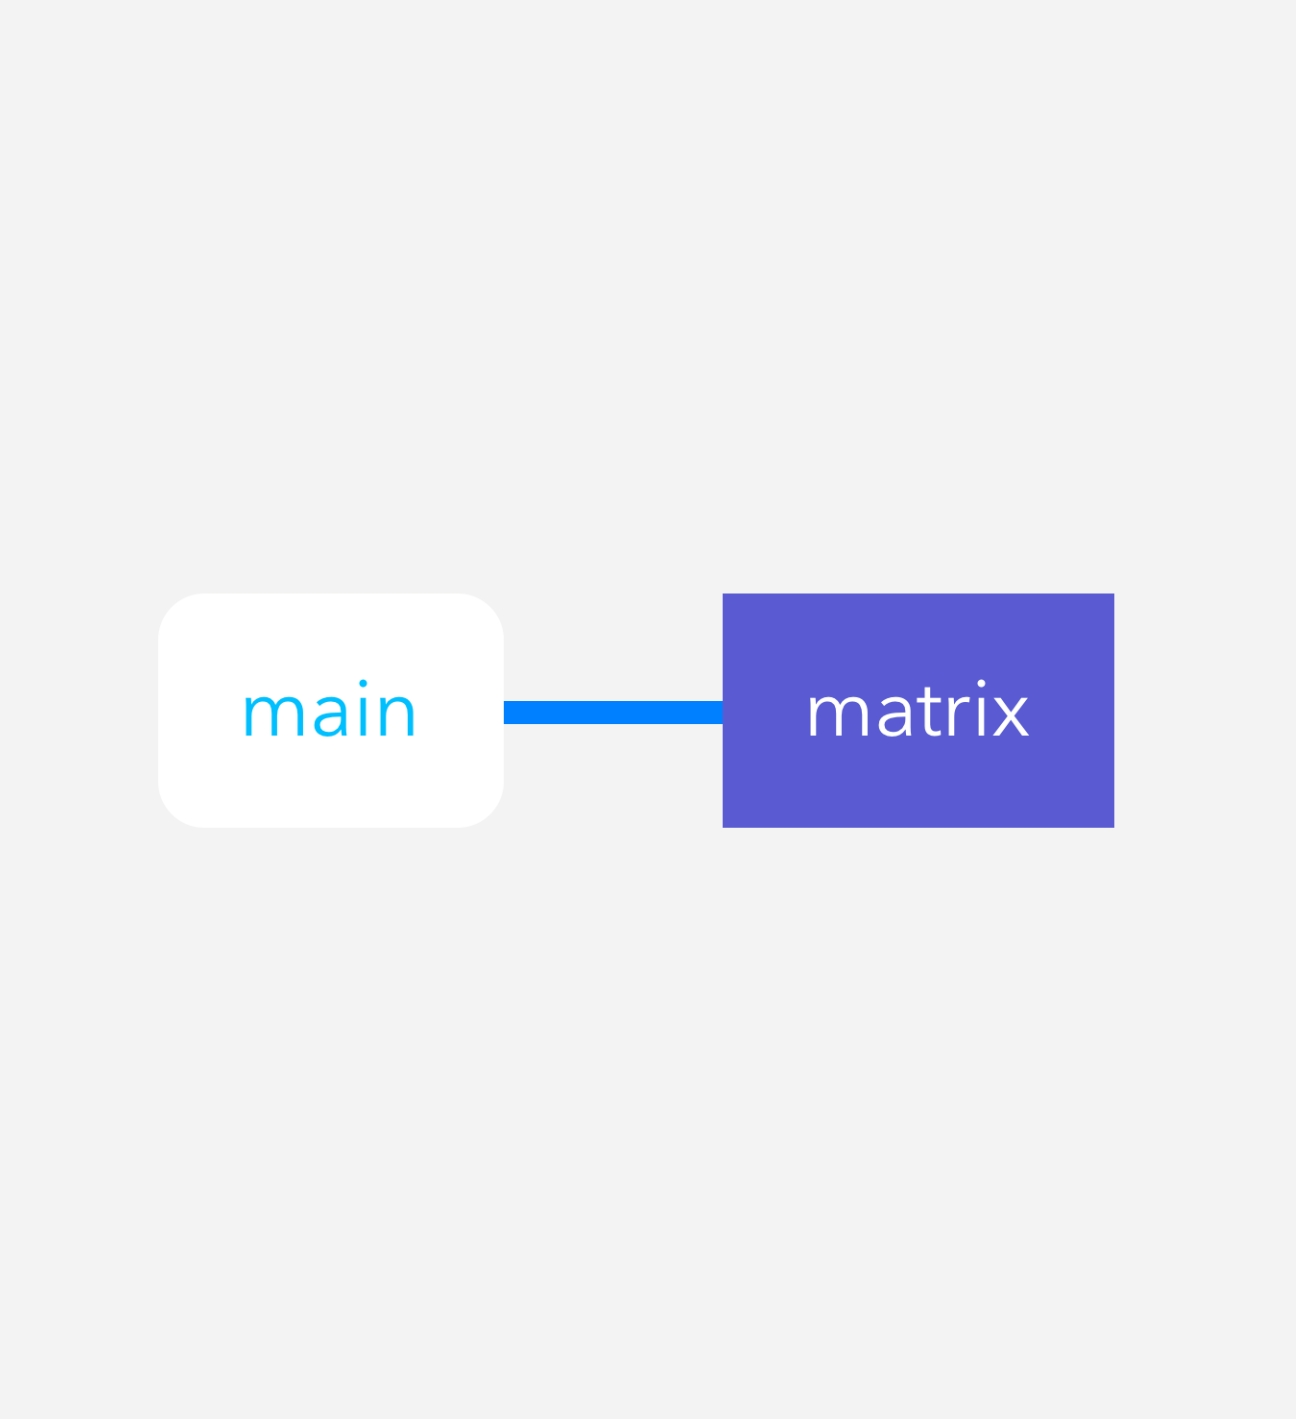
\includegraphics[width=1\textwidth]{./Images/pic3_1.png}

    \caption{程序模块层次关系}

\end{figure}

\section{详细设计}

\subsection{栈的实现}

三元组设计中基本操作的伪代码算法如下:
\begin{lstlisting}[language={C},
    numbers=left,
    numberstyle=\tiny\consolas,
    basicstyle=\small\consolas]
// 初始化矩阵
void initMatrix(Matrix * a, int n, int m)
{
    a->n <- n;
    a->m <- m;
    a->tot <- 0;
    if (a->pos内存分配失败)
        异常退出
    a->sizeOfMatrix <- MATRIXINCREASESIZE;
    if (a->data内存分配失败)
        异常退出
}
    
// 扩展矩阵的存储空间
void expandMatrix(Matrix * c)
{
    // 分配更多存储空间
    if (c->data内存分配失败)
        异常退出
    c->sizeOfMatrix <- c->sizeOfMatrix + MATRIXINCREASESIZE
}

// 把由一维数组存储的矩阵转化为由三元组表存储的矩阵
Matrix array2Matrix(int n, int m, int val[])
{
    定义矩阵 a 并初始化
    for (int i <- 1; i <= n; ++i)
    {
        a.pos[i] <- a.tot + 1
        for (int j <- 1; j <= m; ++j)
        {
            if (val[(i - 1) * m + j]不为空)
            {
                if (矩阵a的存储空间不足)
                    扩展矩阵a的存储空间
                a.data[++a.tot] <- (Tuple) {i, j, val[(i - 1) * m + j]}
            }
        }
    }
    a.pos[n + 1] <- a.tot + 1
    返回 a
}

// 两个矩阵相加
Matrix addMatrix(Matrix a, Matrix b)
{
    if (两个矩阵的行列大小不相等) 
        异常退出
    定义矩阵 c 并初始化
    if (有一个矩阵为空)
        返回空矩阵c
    for (int i <- 1; i 小于等于 a.n; ++i)
    {
        c.pos[i] <- c.tot + 1
        定义整型 p1 <- a.pos[i] 
        定义整型 p2 <- b.pos[i]
        while (p1 小于 a.pos[i + 1] 或 p2 小于 b.pos[i + 1]) // 枚举a矩阵和b矩阵第i行的非零元素
        {
            定义临时整型tempj,tempy // 用于记录c矩阵中每一个位置加法的结果
            if (b矩阵本行没有元素或者a矩阵非零元素列数小于b矩阵非零元素的列数) 
            {
                c[i][j] <- a[i][j]
            }
            else if (a矩阵本行没有元素或者b矩阵非零元素列数小于a矩阵非零元素的列数) 
            {
                c[i][j] <- b[i][j]
            }
            else 
            {
                c[i][j] <- a[i][j]+b[i][j]
            }
            if (c[i][j]不为0)
            {
                if (矩阵c存储空间不足)
                    扩展矩阵的存储空间
                c.data[++c.tot] <- (Tuple) {i, tempj, tempv}
        }
    }
    c.pos[c.n + 1] <- c.tot + 1
    返回 c
}

// 两个矩阵相乘
Matrix mulMatrix(Matrix a, Matrix b)
{
    if (第一个矩阵的列数不等于第二个矩阵的行数) // 两个矩阵不可相乘
        异常退出
    定义矩阵 c 并初始化
    if (有一个矩阵为空)
        返回空矩阵c
    定义临时数组temp并分配内存 // 临时数组,用于记录c矩阵中每一行的结果
    for (int i <- 1; i 小于等于 a.n; ++i)
    {
        memset(temp, 0, (a.m + 1) * sizeof(int));
        c.pos[i] <- c.tot + 1;
        for (int p <- a.pos[i]; p 小于 a.pos[i + 1]; ++p) // 枚举a矩阵第i行的非零元素
        {
            int k <- a.data[p].j // a矩阵的该非零元素为a[i][k]
            for (int q <- b.pos[k]; q 小于 b.pos[k + 1]; ++q) // 枚举b矩阵第k行的非零元素
            {
                int j <- b.data[q].j // b矩阵的该非零元素为b[k][j]
                c[i][j] <- c[i][j] + a[i][k]*b[k][j]
            }
        }
        for (int j <- 1; j 小于等于 a.m; ++j)
        {
            if (c[i][j]不等于0) 
                继续下一轮循环
                if (矩阵c存储空间不足)
                扩展矩阵的存储空间
            c.data[++c.tot] <- (Tuple) {i, tempj, tempv}
        }
    }
    c.pos[c.n + 1] <- c.tot + 1;
    释放临时数组temp
    返回 c
}

// 把由三元组表存储的矩阵转化为由一维数组存储的矩阵
void matrix2Array(Matrix a, int val[])
{
    memset(val, 0, sizeof(int) * (a.n * a.m + 1));
    for (int i <- 1; i 小于等于 a.tot; ++i)
        val[(a.data[i].i - 1) * a.m + a.data[i].j] <- a.data[i].val; // a[i][j]存储在val[(i-1]*m+j]中
}

// 释放矩阵空间
void destroyMatrix(Matrix * a)
{
    释放a->pos
    释放a->data
    a->n <- 0
    a->m <- 0
    a->tot <- 0
    a->sizeOfMatrix <- 0
}

\end{lstlisting}

\subsection{函数的调用关系图}

函数调用关系图如图2。

\begin{figure}[htbp]
    
    \centering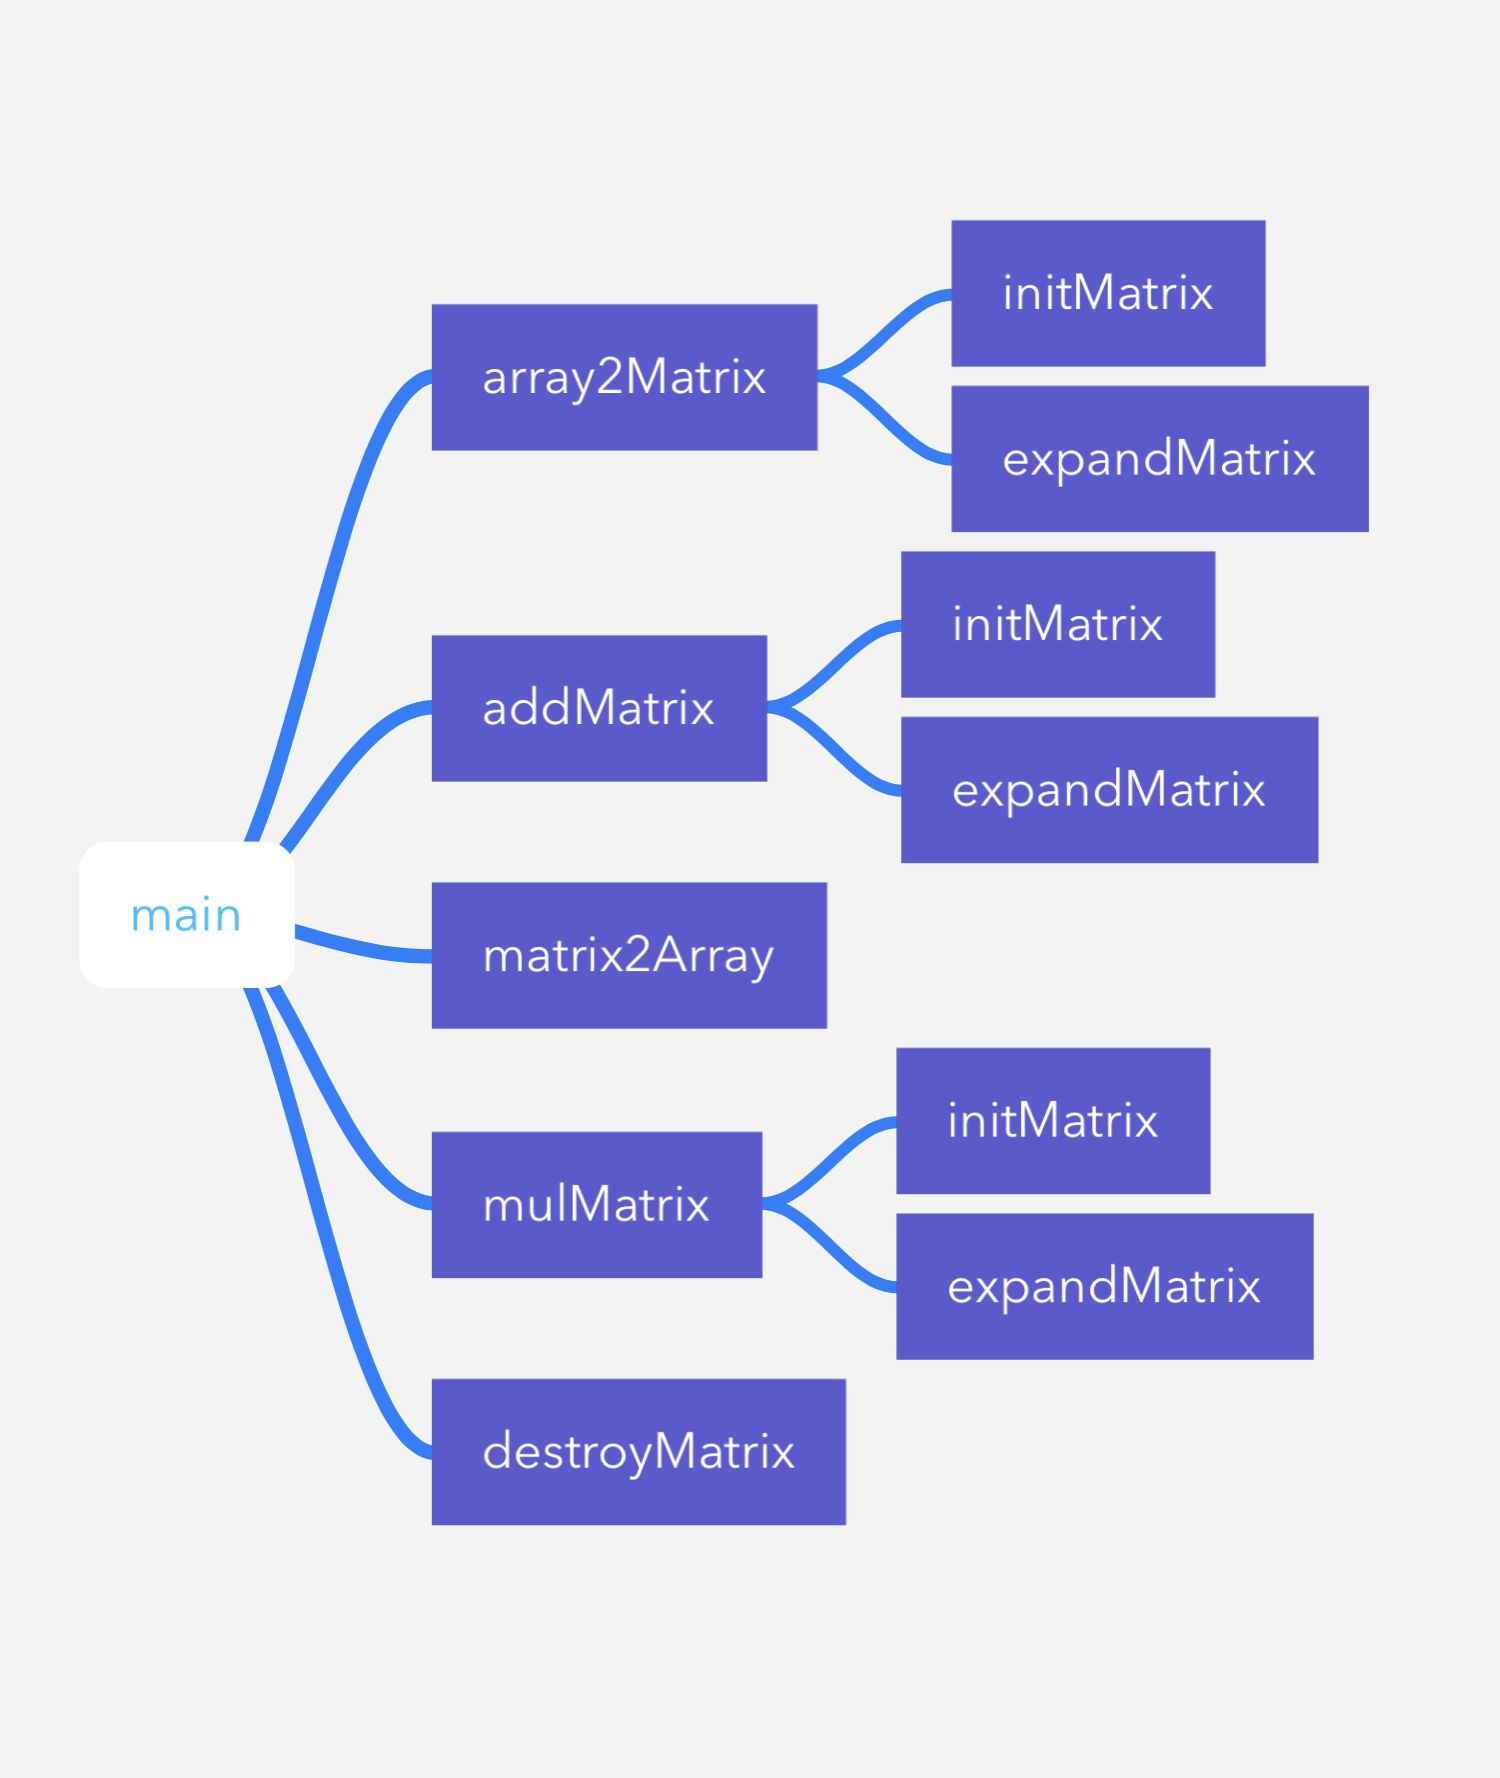
\includegraphics[width=0.4\textwidth]{./Images/pic3_2.png}
    
    \caption{函数调用关系图}
    
\end{figure}

\section{调试分析报告}

\subsection{调试过程中遇到的问题和思考}


\subsection{设计实现的回顾讨论}


\subsection{算法复杂度分析}


\subsection{改进设想的经验和体会}

\subsubsection{改进1}


\begin{lstlisting}[language={C},
    numbers=left,
    numberstyle=\tiny\consolas,
    basicstyle=\small\consolas]

\end{lstlisting}



\section{用户使用说明}

\subsection{栈和队列的顺序实现}

使用gcc编译生成可执行文件。

\begin{lstlisting}[language={bash},
    basicstyle=\small\consolas]
gcc -o main -std=c11 main.c stack.c queue.c
\end{lstlisting}

执行可执行文件:

\begin{lstlisting}[language={bash},
    basicstyle=\small\consolas]
./main
\end{lstlisting}

在Windows cmd下:

\begin{lstlisting}[language={bash},
    basicstyle=\small\consolas]
main
\end{lstlisting}

之后通过标准输入输入数据,输入格式参考1.2节的输入描述,结果通过标准输出返回。如果输入合法并且程序正常运行结束,主函数返回值为0。

\subsection{栈和队列的链表实现}

使用gcc编译生成可执行文件。

\begin{lstlisting}[language={bash},
    basicstyle=\small\consolas]
gcc -o main -std=c11 main1.c stack.c queuelist.c
\end{lstlisting}

执行可执行文件:

\begin{lstlisting}[language={bash},
    basicstyle=\small\consolas]
./main
\end{lstlisting}

在Windows cmd下:

\begin{lstlisting}[language={bash},
    basicstyle=\small\consolas]
main
\end{lstlisting}

之后通过标准输入输入数据,输入格式参考1.2节的输入描述,结果通过标准输出返回。如果输入合法并且程序正常运行结束,主函数返回值为0。

\section{测试结果}

本题的两种实现方式均通过以下测试。

测试环节分为三个步骤。

\subsection{测试第一部分}

对1.4节给出的样例进行测试。

\subsection{测试第二部分}

测试边界条件。

【输入】

\begin{lstlisting}[
    basicstyle=\small\consolas]
#
\end{lstlisting}

(认为空串是回文串)

【输出】

\begin{lstlisting}[
    basicstyle=\small\consolas]
YES
\end{lstlisting}

【输入】

\begin{lstlisting}[
    basicstyle=\small\consolas]
1#
\end{lstlisting}

【输出】

\begin{lstlisting}[
    basicstyle=\small\consolas]
YES
\end{lstlisting}

【输入】

\begin{lstlisting}[
    basicstyle=\small\consolas]
00#
\end{lstlisting}

【输出】

\begin{lstlisting}[
    basicstyle=\small\consolas]
YES
\end{lstlisting}

\subsection{测试第三部分}

将原解法与4.4.1节改进解法比对。

测试在macOS\ Catalina\ 10.15.6下进行。

在$LEN<=10$,$LEN<=1000$,$LEN<=1000000$的范围下分别随机生成1000组测试数据,分别传入main和test,并且比对两程序的输出。

3000组数据中两程序的输出均相同。

数据生成程序(testing/data.cpp)如下:

\begin{lstlisting}[language={C++},
    numbers=left,
    numberstyle=\tiny\consolas,
    basicstyle=\small\consolas]
#include <bits/stdc++.h>

using namespace std;

const int LEN = 1e6;
char a[LEN + 10];

int main()
{
    srand(time(0));
    int n = rand() % LEN + 1;
    for (int i = 1; i <= n / 2; ++i)
        printf("%c", a[i] = rand() % 26 + 'a');
    if (rand() % 2 == 1)
    {
        for (int i = 1; i <= n / 2; ++i)
            printf("%c", a[i]);
    }
    else
    {
        for (int i = n / 2; i >= 1; --i)
            printf("%c", a[i]);
    }
    puts("#");
    return 0;
}
\end{lstlisting}

比对脚本(testing/chk.sh)如下:

\begin{lstlisting}[language={bash},
    numbers=left,
    numberstyle=\tiny\consolas,
    basicstyle=\small\consolas]
for i in {1..100}
do
    sleep 1
    ./data >in.in
    ./main <in.in >out.out
    ./test <in.in >out1.out
    if ! diff out.out out1.out
    then
        break
    fi
    echo "Correct"
done
\end{lstlisting}

\end{document}
